The convolutional VAE is implemented in the file \texttt{convolutional\_vae.py} by extending the encoder and decoder of the original VAE with convolutional layers. The encoder portion of the network uses a series of convolutional layers (Conv2d) with kernel size 4, stride 2, and padding 1. These layers take in a single channel image and output 32, 64, and 128 channels respectively. Since the stride is 2, the output of each layer is half the size of the input. The output of these layers is then flattened and passed through a linear layer with 100 units to produce the encoded representation of the input image. This encoded representation is then passed through two linear layers to produce the mean and variance of the latent space, respectively.

The decoder portion of the network takes in the latent space and passes it through a linear layer with 100 units to produce the decoder's input. This input is then passed through a linear layer with 12833 units, which reshapes the input to match the shape of the output from the encoder. The output is then passed through a series of transposed convolutional layers (ConvTranspose2d) with kernel size 4, stride 2, and padding 1, which take in 128, 64, and 32 channels respectively and output a single channel image. The output of the final layer is passed through a sigmoid activation function to produce the final output image. We expect that the quality of the model will be better than the original VAE since convolutional layers are usally more suited for image data and can capture spatial hierarchies and patterns in the data that linear layers are not able to.

The parameters of the network were estimated using the Adam optimizer and the ELBO loss. ELBO is the sum of two terms: the reconstruction loss (BCE) and the KL-divergence. By minimizing this loss, the VAE is able to learn a good approximation of the true posterior, and generate realistic samples from the learned latent space. Both models were trained for 100 epochs with a batch size of 128. The models were trained with a learning rate of 0.0005 and a weight decay of 0. We trained both models on the MNIST dataset with a varying number of latent dimensions. The results are shown in Figure \ref{fig:vaeloss}.

\begin{figure}[H]
\centering
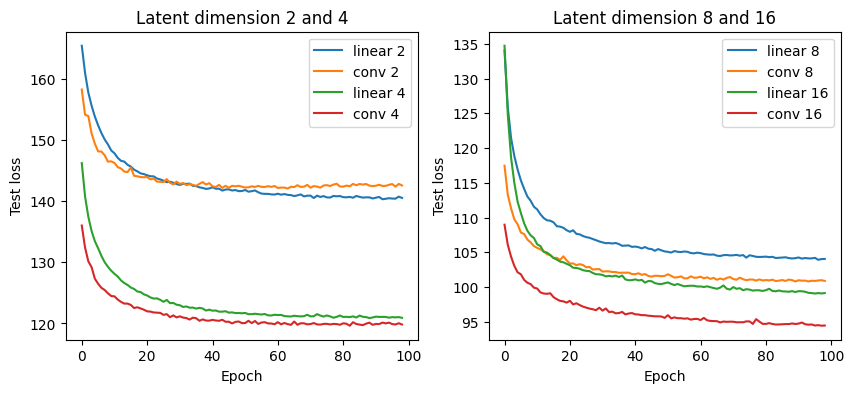
\includegraphics[width=\textwidth]{images/test_loss.png}
\caption{ELBO reconstruction loss on test set for VAE and Convolutional VAE with varying number of latent dimensions.}
\label{fig:vaeloss}
\end{figure}

\begin{table}
\centering
\begin{tabular}{|c|c|c|}
\hline
\multicolumn{1}{|c|}{\textbf{Latent Dimensions}} & \multicolumn{1}{c|}{\textbf{Original VAE}} & \multicolumn{1}{c|}{\textbf{Convolutional VAE}} \\ \hline
\multicolumn{1}{|c|}{2} & \multicolumn{1}{c|}{140.54} & \multicolumn{1}{c|}{142.58}  \\ \hline
\multicolumn{1}{|c|}{4} & \multicolumn{1}{c|}{120.92} & \multicolumn{1}{c|}{119.83}  \\ \hline
\multicolumn{1}{|c|}{8} & \multicolumn{1}{c|}{104.03} & \multicolumn{1}{c|}{100.86}  \\ \hline
\multicolumn{1}{|c|}{16} & \multicolumn{1}{c|}{99.117} & \multicolumn{1}{c|}{94.446}  \\ \hline
\multicolumn{1}{|c|}{32} & \multicolumn{1}{c|}{99.136} & \multicolumn{1}{c|}{94.434}  \\ \hline
\end{tabular}
\vspace*{0.5cm}
\caption{ELBO reconstruction loss on test set for VAE and Convolutional VAE with varying number of latent dimensions.}
\label{tab:vaeloss}
\end{table}

We see that the original VAE actually performs better than the convolutional VAE for the 2 dimensional latent space. The difference is not significant, but it is still interesting to note. One explanation for this would be that the original VAE can learn a simpler, more linear structure of the data when the latent dimensions are low, and this structure is sufficient to capture the information in the MNIST dataset. However, as the latent dimensions rise, the initial VAE can find it harder to understand a more intricate, non-linear data structure.

Contrarily, convolutional VAE can learn spatial hierarchies in the data and is meant to handle high-dimensional data, such as images. As a result, it can still function more effectively when the latent dimensions are larger. Hence, the convolutional VAE performs better than the original VAE for all other latent dimensions (4, 8, 16, 32).

The difference between 16 and 32 latent dimensions for each of the models among themselves is very small, hence why we don't show results for 32 latent dimensions in the graph. It is suprising that we did not see a significant improvement when going from 16 to 32 latent dimensions in the convolutional VAE. We think that this is because the convolutional VAE is not large enough to capture the information in the data. The convolutional VAE is a relatively small network, and it is possible that it is not able to learn the complex structure of the data with 32 latent dimensions.

We are fairly confident that a convolutional VAE could perform better than the original VAE when the latent dimensions are 2, if we adjust the capacity of the network and use techniques such as batch normalization and dropout. If we increase the size of the network, we also expect that the convolutional VAE will have a bigger difference in performance between 16 and 32 latent dimensions. 

We can also compare the performance of the original VAE and convolutional VAE by looking at the reconstructions visualized in Figure \ref{fig:reconstructions}. We use the models trained with 16 latent dimensions to generate the reconstructions. We see that the original VAE is able to reconstruct the images fairly well, but the convolutional VAE is able to reconstruct the images more accurately.

\begin{figure}[H]
\centering
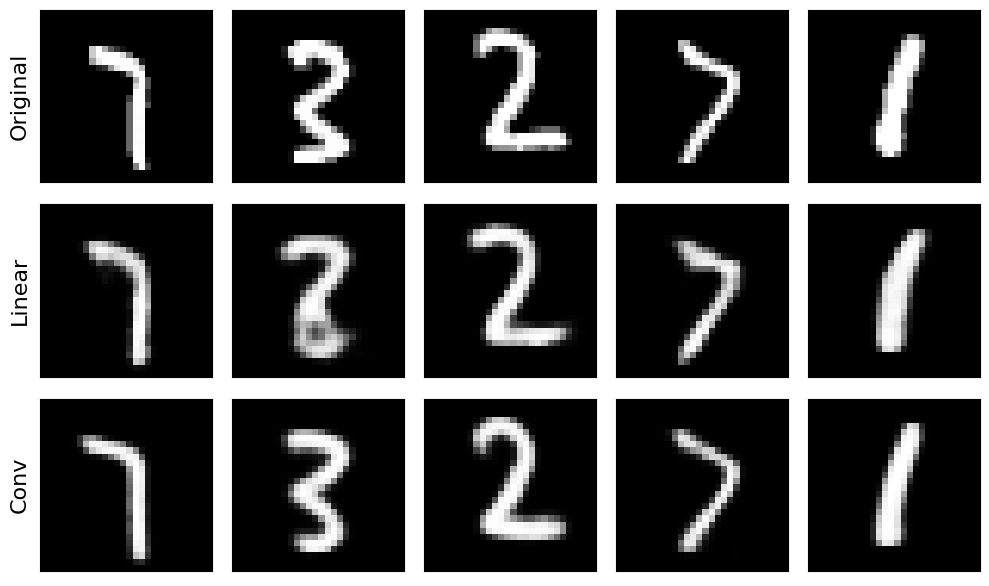
\includegraphics[width=\textwidth]{images/reconstructions.png}
\caption{Reconstructions of the original VAE and convolutional VAE.}
\label{fig:reconstructions}
\end{figure}
